\documentclass{handout}

%\SetInstructor{Capt Steven Beyer}
\SetCourseTitle{ECE210: Introduction to Electrical and Computer Engineering}
\SetHandoutTitle{Build Robot}

%\ShowAllBlanks

\usepackage[obeyspaces]{url}

\graphicspath{{./figs/}}

%\showsoln \setsolncolor{red}

\begin{document}
	%	\footnotetext{Examples are abstracted from Tutorials Point, "Arduino", 2019, accessed Feb 18, 2019. [Online]. Available: https://www.tutorialspoint.com/arduino/index.htm}
	\maketitle
	
	\section{Objectives.} 
	\begin{enumerate}
		\item Demonstrate the ability to build a robotics system using Electrical and Computer Engineering (ECE) fundamentals such as soldering, assembly, and fabrication.
		\item Troubleshoot ECE applications utilizing modern test equipment.
	\end{enumerate}
	
	\section{Materials.}
	\begin{enumerate}
		\item Soldered Printed Circuit Board (PCB)
		\item Arduino Uno
		\item 3D-printed structural pieces (A-D)
		\item 2 - DC motors
		\item 2 - wheels
		\item 2 - tires (note left and right are different)
		\item 1 - Battery pack
		\item Jumper wire pack
		\item 1 - Switch
		\item 3 - IR sensors
		\item 1 - QTR-8RC Reflectance Sensor Array
		\item 1 - 1x11 90$^o$ header
		\item 8 - hex standoffs (4 short and 4 long)
		\item Bolts
		\begin{enumerate}
			\item 6 - \# 4-40 x 1"
			\begin{enumerate}
				\item 4 for motors
				\item 2 for connecting A and B
			\end{enumerate}
			\item 8 - \# 4-40 x 1/4"
			\begin{enumerate}
				\item 8 for connecting standoffs to layers
			\end{enumerate}
			\item 10 - \# 2-56 x 1/4"
			\begin{enumerate}
				\item 2 for line sensors
				\item 6 for IR sensors
				\item 2 for wheels
			\end{enumerate}
		\end{enumerate}
		\item Nuts
		\begin{enumerate}
			\item 6 - \# 4-40
			\item 8 - \# 2-56
		\end{enumerate}
	\end{enumerate}
	\newpage
\clearpage
\pagebreak
	
	\section{Layer A - Base Layer.}
	\begin{enumerate}
		\item Remove the support from Layer A.
		\item Place the PCB on the printed spacers with the ``Beyer" printed text towards the rounded edge.
		
		\begin{figure} [H]
			\centering
			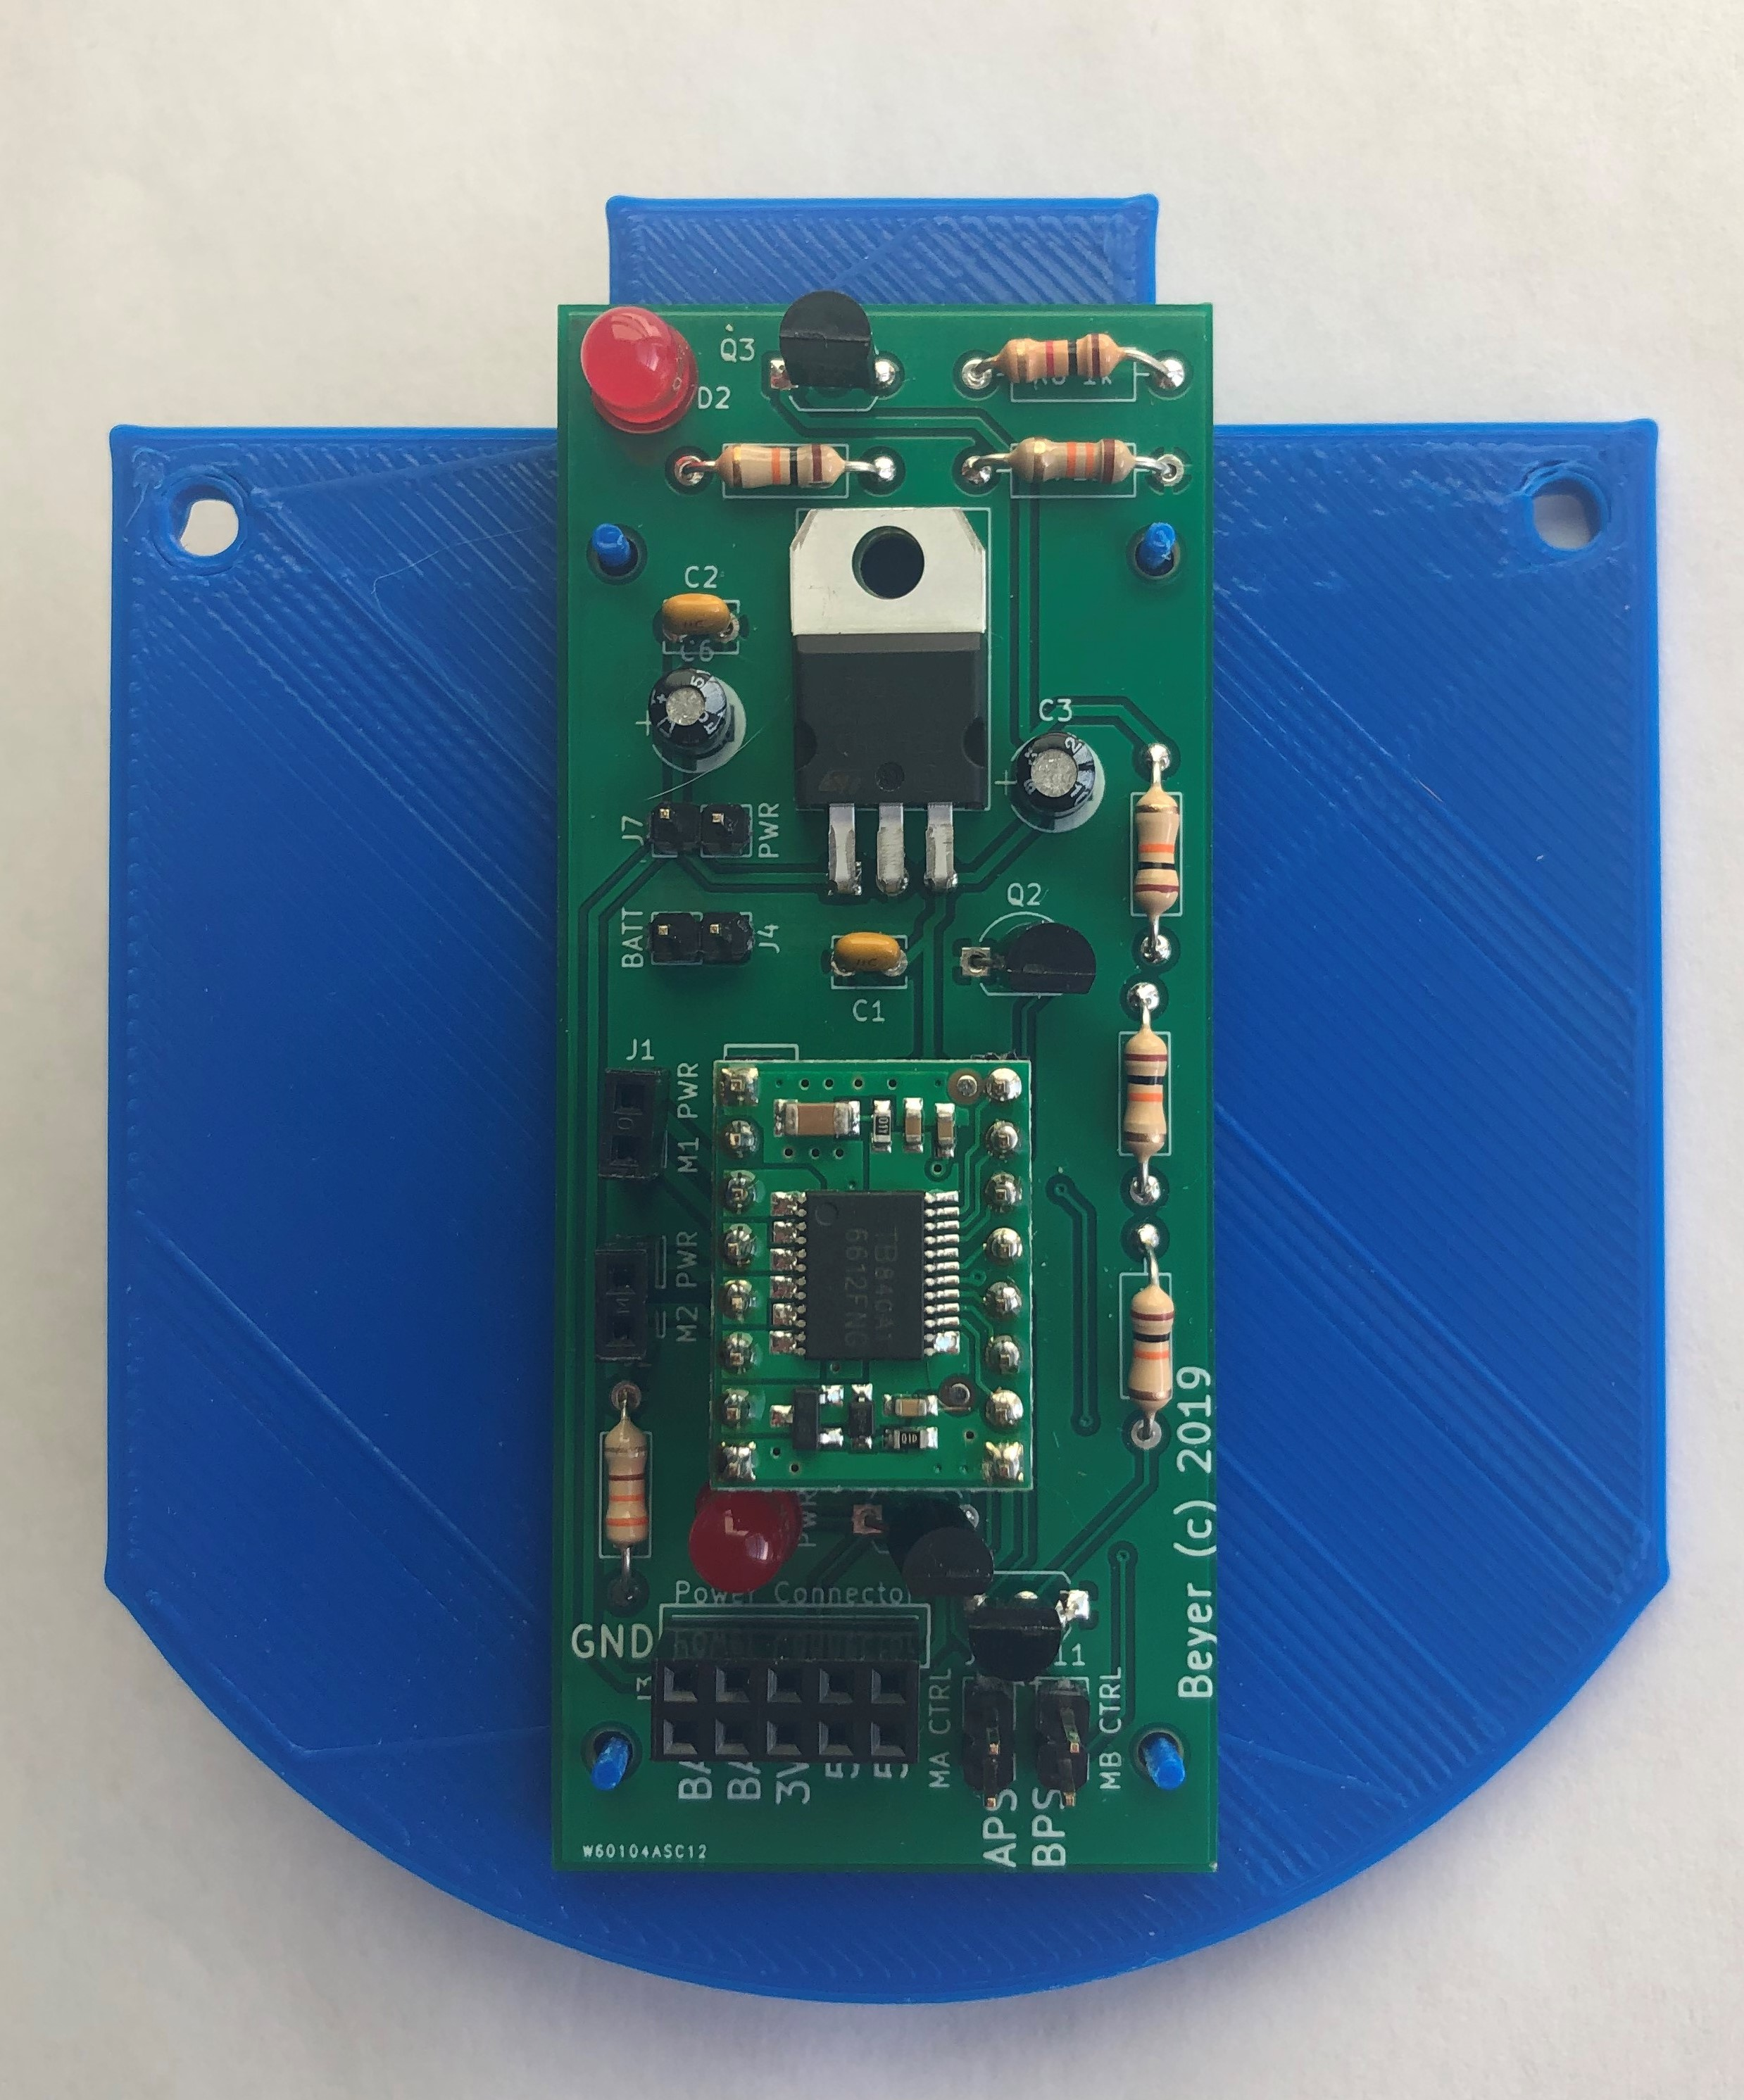
\includegraphics[width=.75\textwidth]{1.jpg}
		\end{figure}
	
		\item Solder the 1 x 11 90$^o$ header to the reflectance sensor array with the header opposite of the line sensors
		
		\item Solder a jumper across the $3.3\ V$ bypass.
		
		\item Secure the reflectance sensor array to the line sensor mount using 2 - \#2-56 x 1/4" bolts and nuts.
		
		\begin{figure} [H]
			\centering
			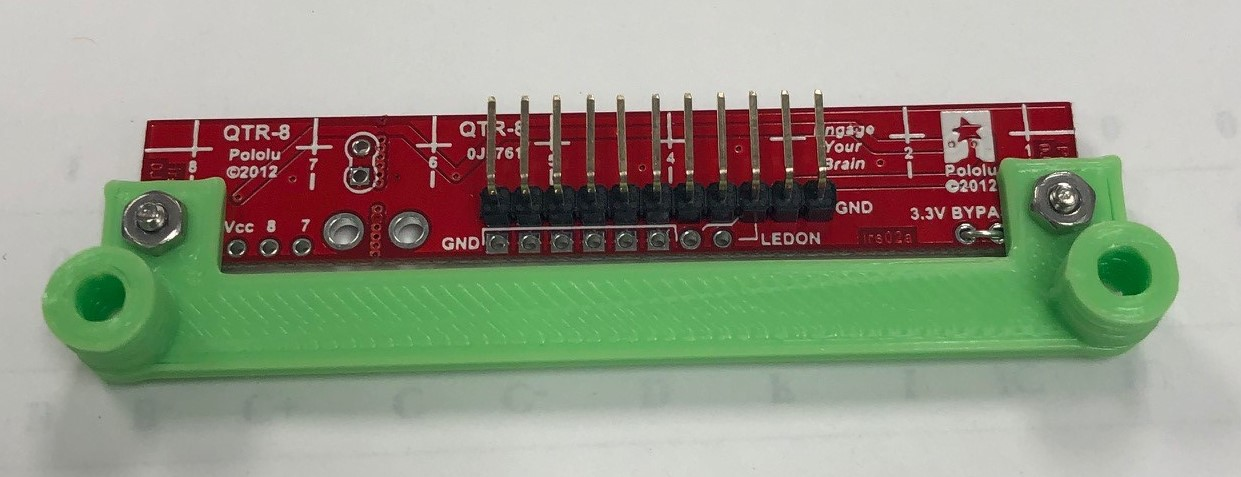
\includegraphics[width=.75\textwidth]{2.jpg}
		\end{figure}
	\end{enumerate}
	
	\section{Layer B - Motor Layer.}
	\begin{enumerate}
		\item Remove the support from Layer B.
		\item Use 4 - \# 4-40 x 1/4" bolts and attach the 4 short hex standoffs to Layer B (outermost holes and opposite of the printed B).
		\item Install the 2 DC motors to Layer B with wires facing inwards. The motors have yellow plastic cases that should be oriented towards the front of Layer B. The white plastic drive shafts should be protruding through the side holes of Layer B. Use 4 - \# 4-40 x 1" bolts and nuts to secure each motor (Ensure the screw heads are to the outside of Layer B).
		
		\begin{figure} [H]
			\centering
			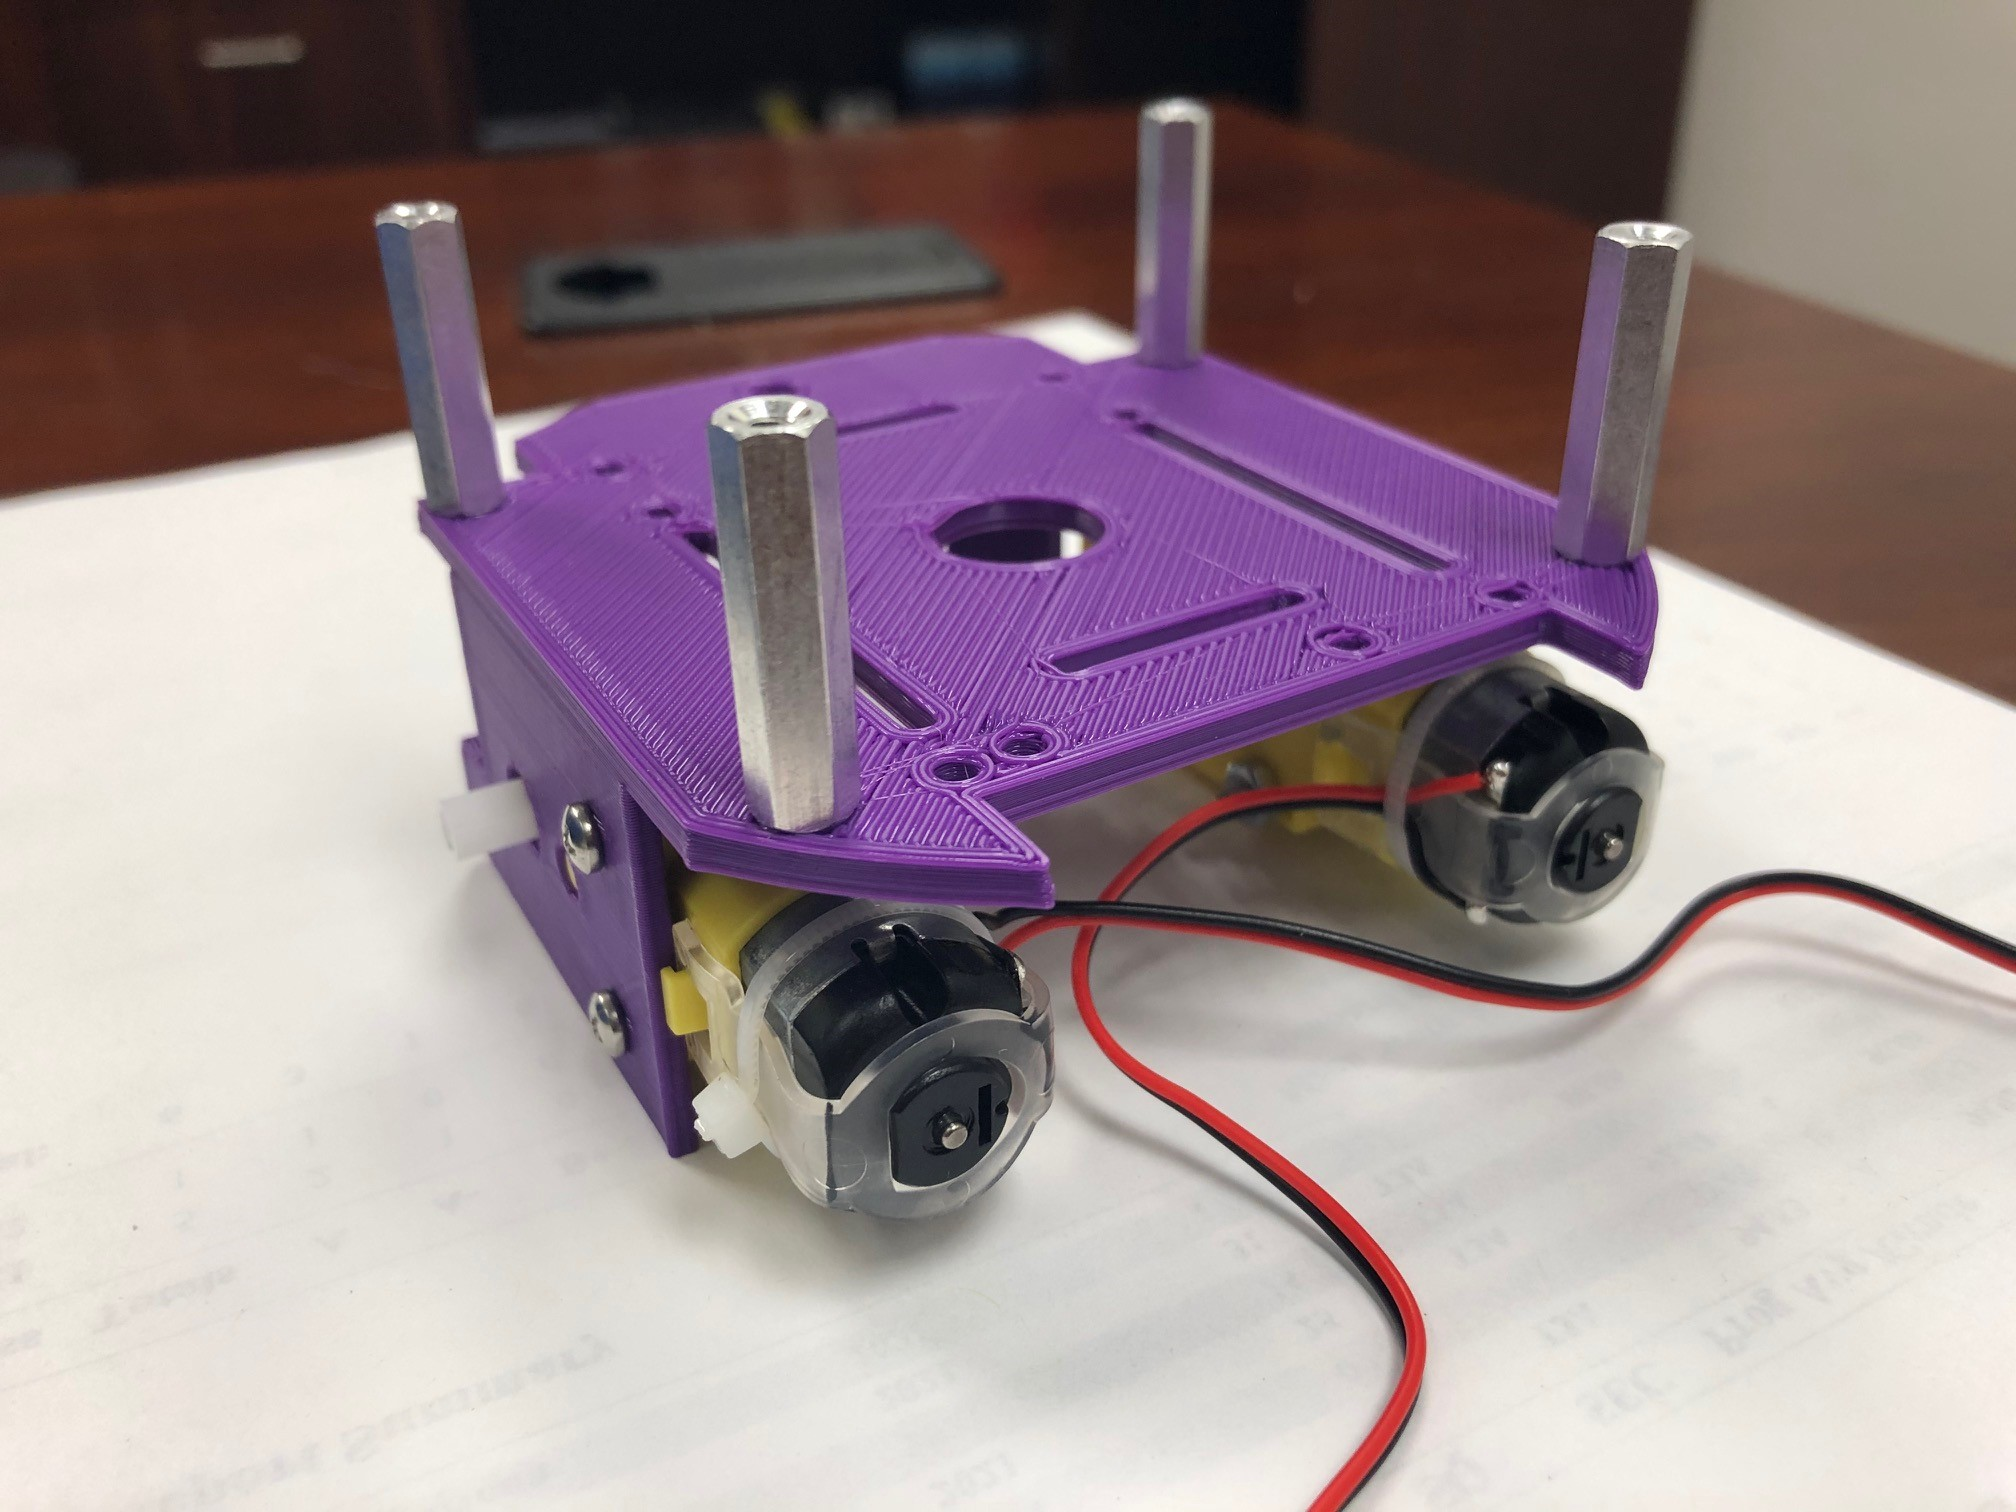
\includegraphics[width=.75\textwidth]{3.jpg}
		\end{figure}
		
		\item \textbf{IR Sensor:} Connect three IR sensors to the sensor mounts on the front of the bot using 6 - \#2-56 x 1/4" bolts and nuts.

		\item Solder three JST IR Sensor cables:
		\begin{itemize}
			\item Solder the three black wires to a single black jumper wire.
			\item Solder the three red wires to a single red jumper wire.
			\item Solder the left IR Sensor's yellow wire to a single green jumper wire.
			\item Solder the center IR Sensor's yellow wire to a single yellow jumper wire.
			\item Solder the right IR Sensor's yellow wire to a single orange jumper wire.
		\end{itemize}
	
		\item \textbf{Switch:} Solder the male ends of two male-to-female jumper wires to the connectors on the switch.
		\item Remove the two nuts and lock washer that came attached to the switch and use one nut to attach it to Layer B in the same direction as the standoffs.
		
		\item \textbf{Wheels:} Attach the wheels by sliding them onto the axles. Use 2 - \# 2-56 x 1/4" bolts to secure the wheels onto the axles.
		
		\begin{figure} [H]
			\centering
			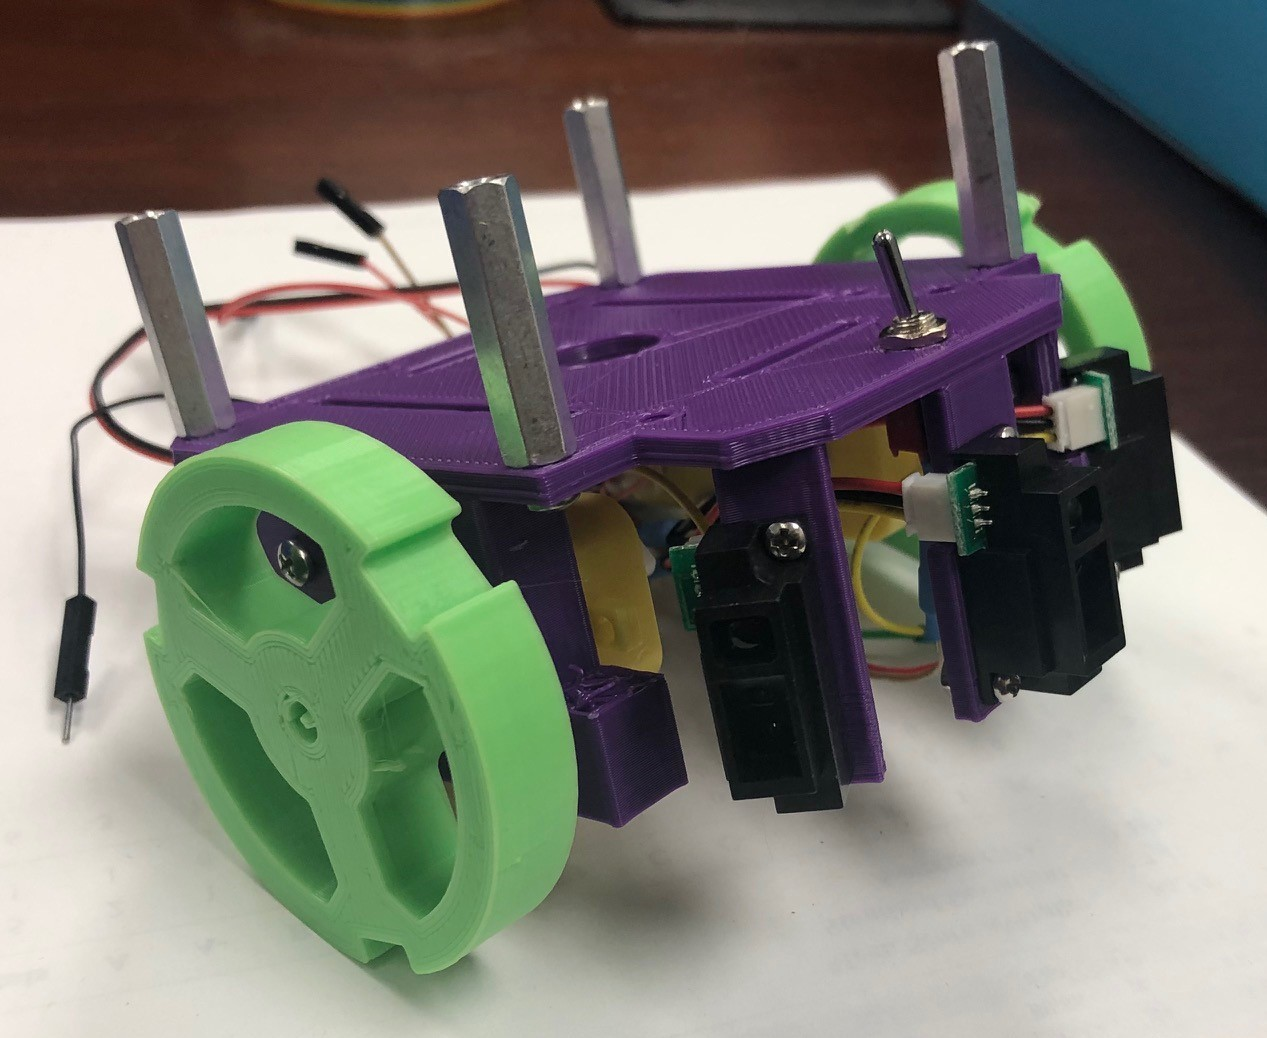
\includegraphics[width=.3\textwidth]{4.jpg}
		\end{figure}
		
		\item \textbf{Battery:} Connect a male to female jumper to the \textit{BATT} headers on the PCB and feed through a slot in Layer B. These wires will connect to the battery and enable the removal of the battery without taking apart the bot.
		
		\begin{figure} [H]
			\centering
			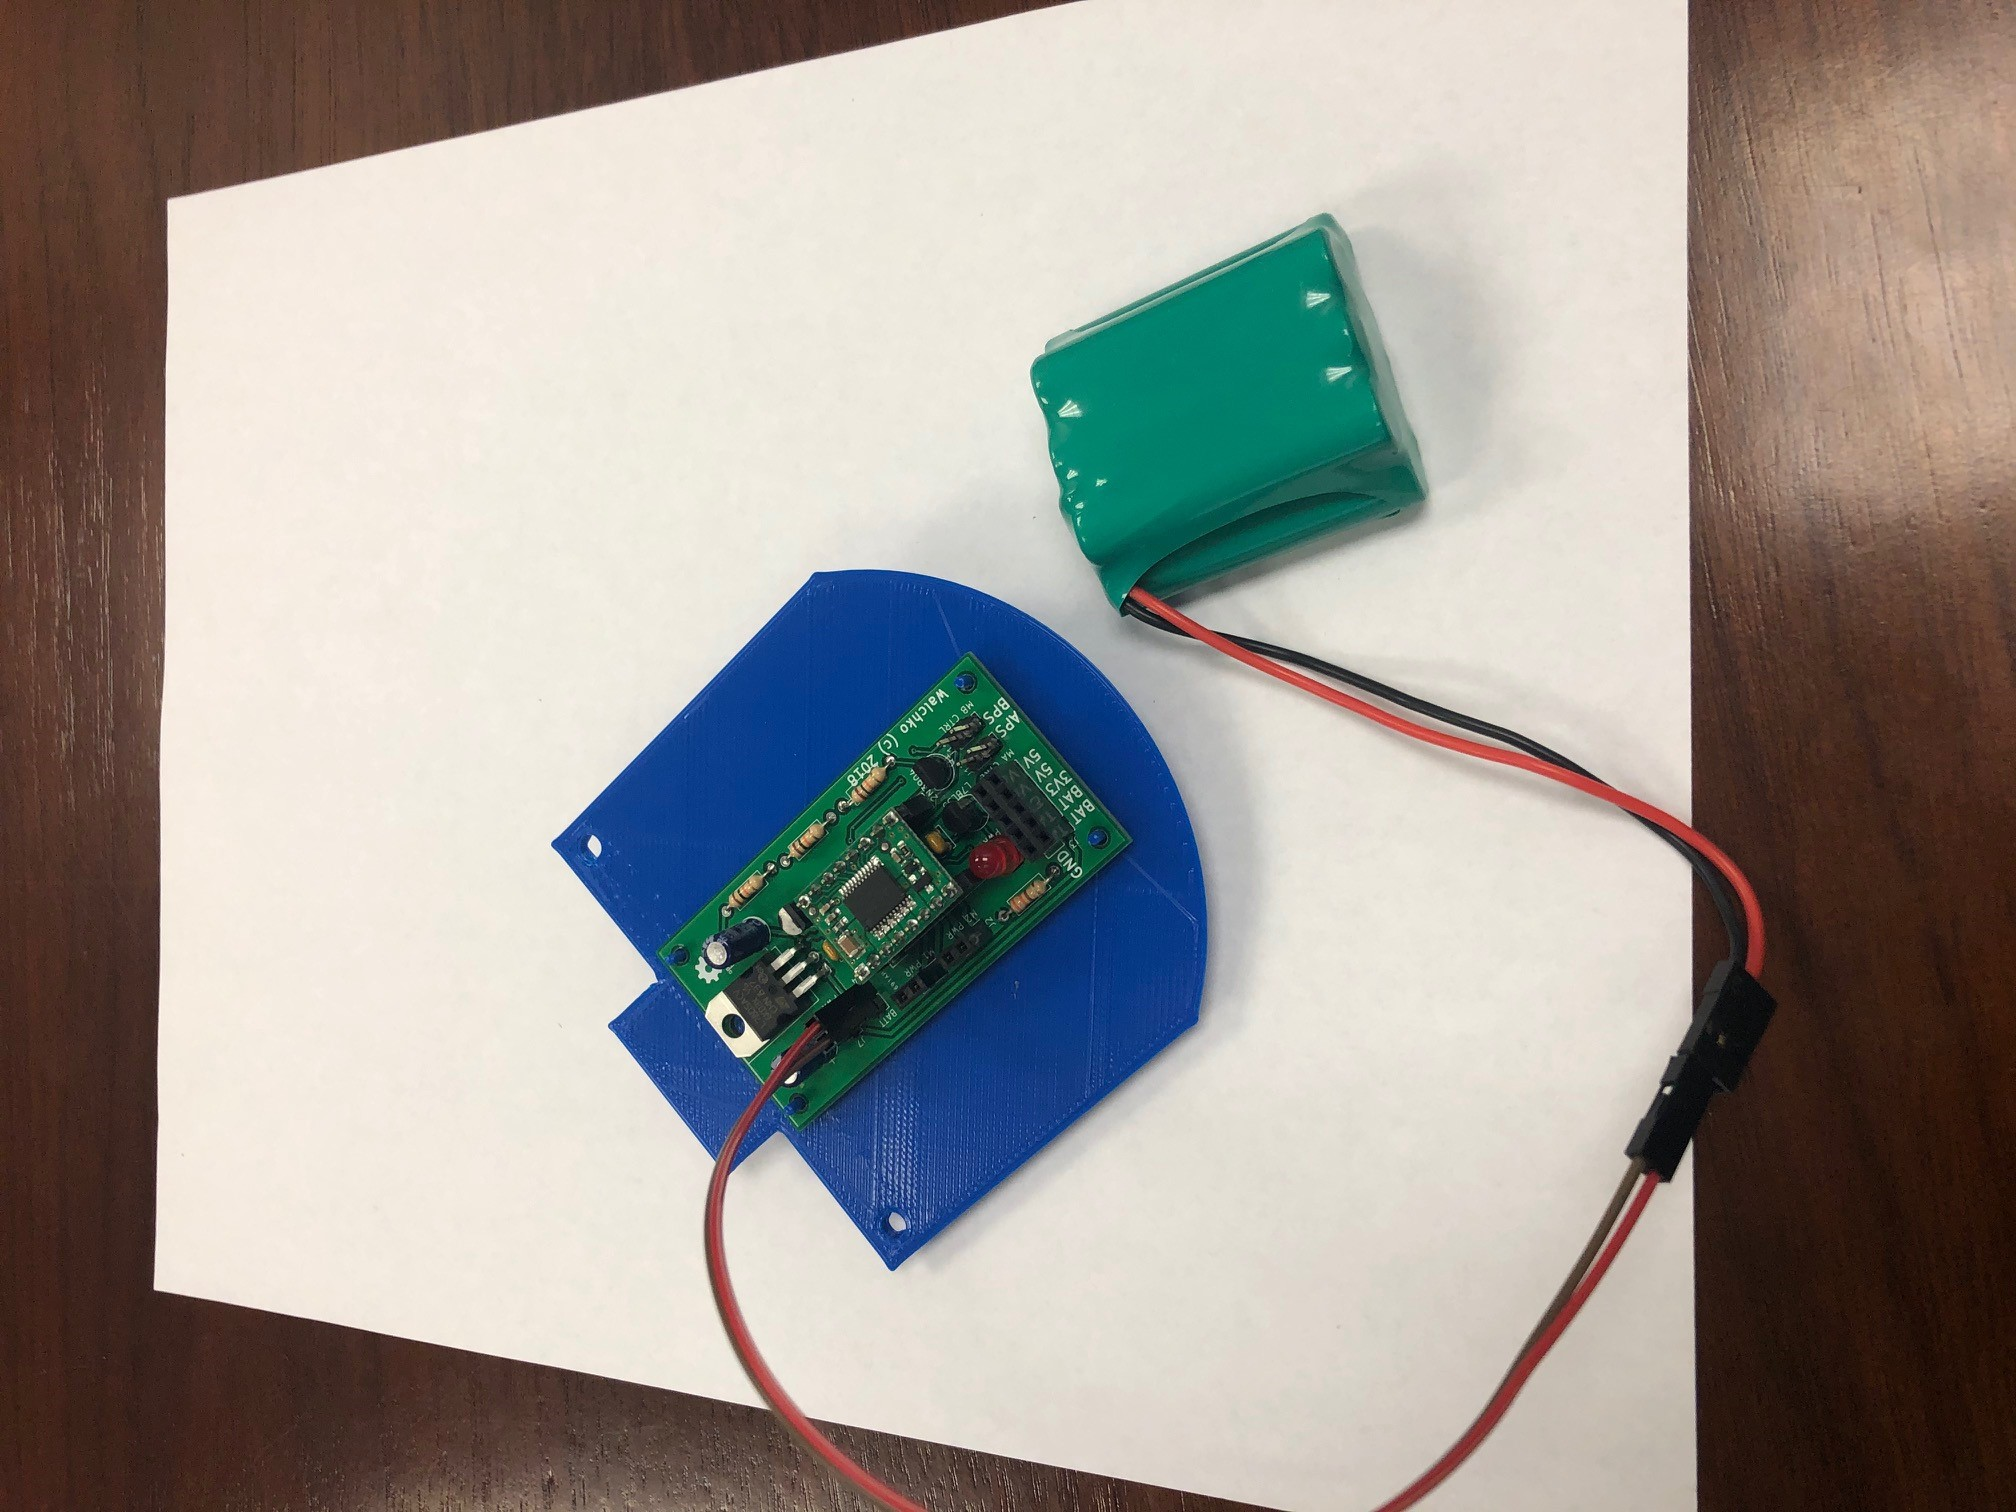
\includegraphics[width=.75\textwidth]{5.jpg}
		\end{figure}
		
		\item \textbf{Testing PCB:} Wire the motors, Arduino, battery, and switch to the PCB as shown in Figure. Download the \path{robot_pcb} folder from \textbf{Teams} (\path{Labs/robot_pcb}). Copy the Motor library from \textbf{Teams} (\path{Labs/Custom Libraries/Motor}) to your documents folder: \\\path{Documents/Arduino/libraries/} Open the \path{robot_pcb.ino} file. Compile and upload to the Arduino. If working correctly, the tires should go forward for 1 second, then left for 1 second, then right for 1 second, then backwards for 1 second. Disconnect the PCB from the Arduino.
		
		\begin{figure} [H]
			\centering
			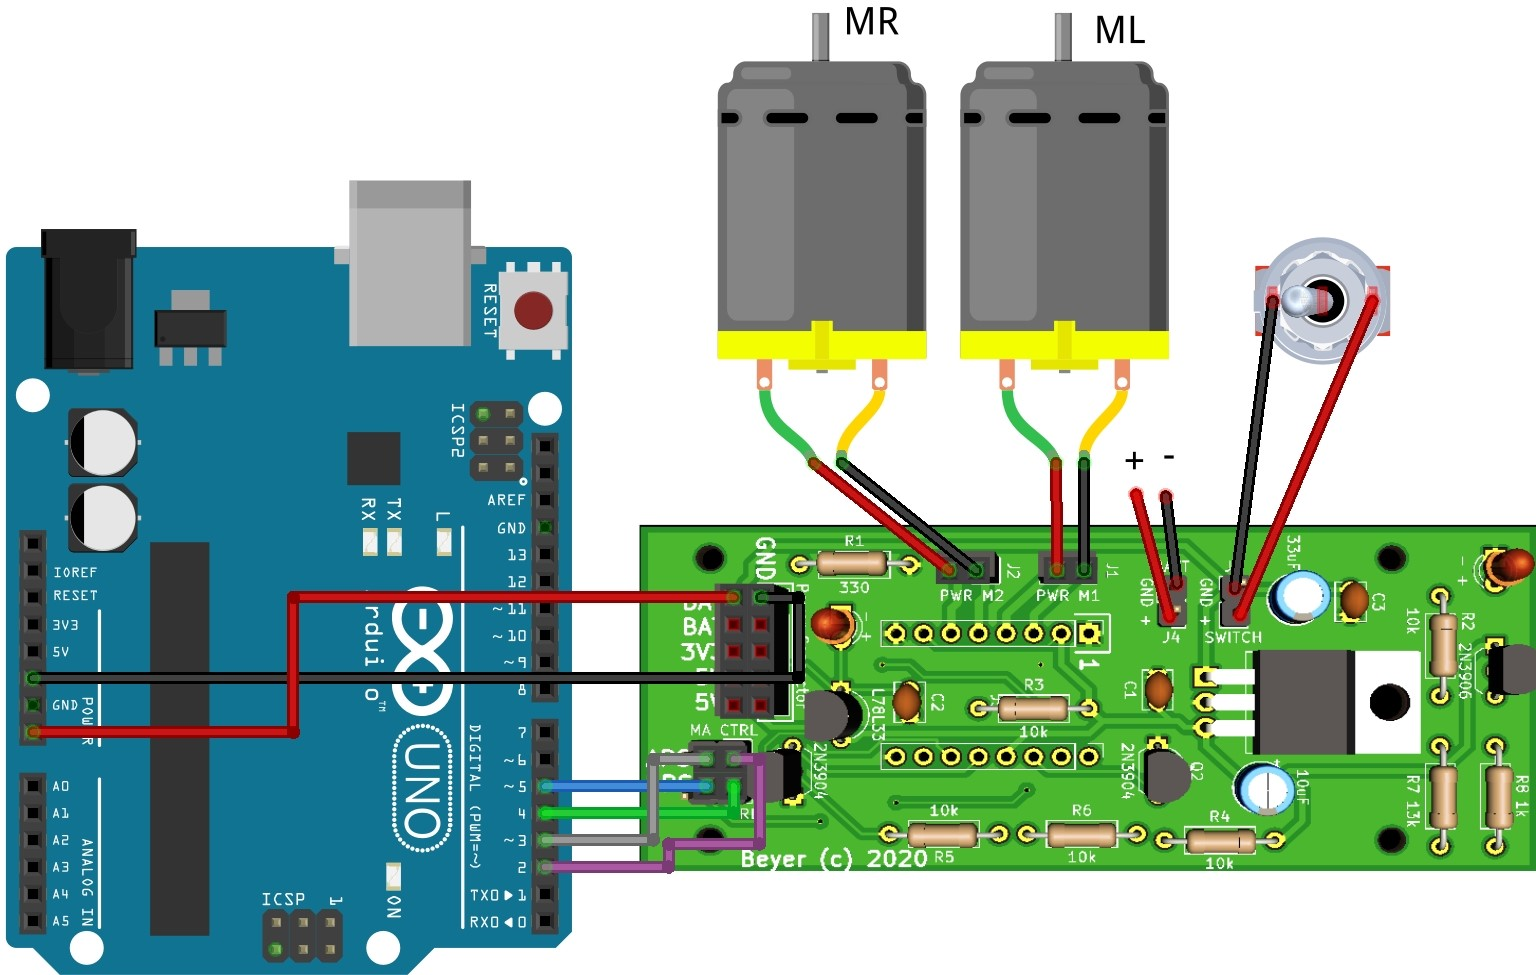
\includegraphics[width=.7\textwidth]{6.jpg}
		\end{figure}
		
		\item Secure the battery to Layer B using velcro.
		
		\begin{figure} [H]
			\centering
			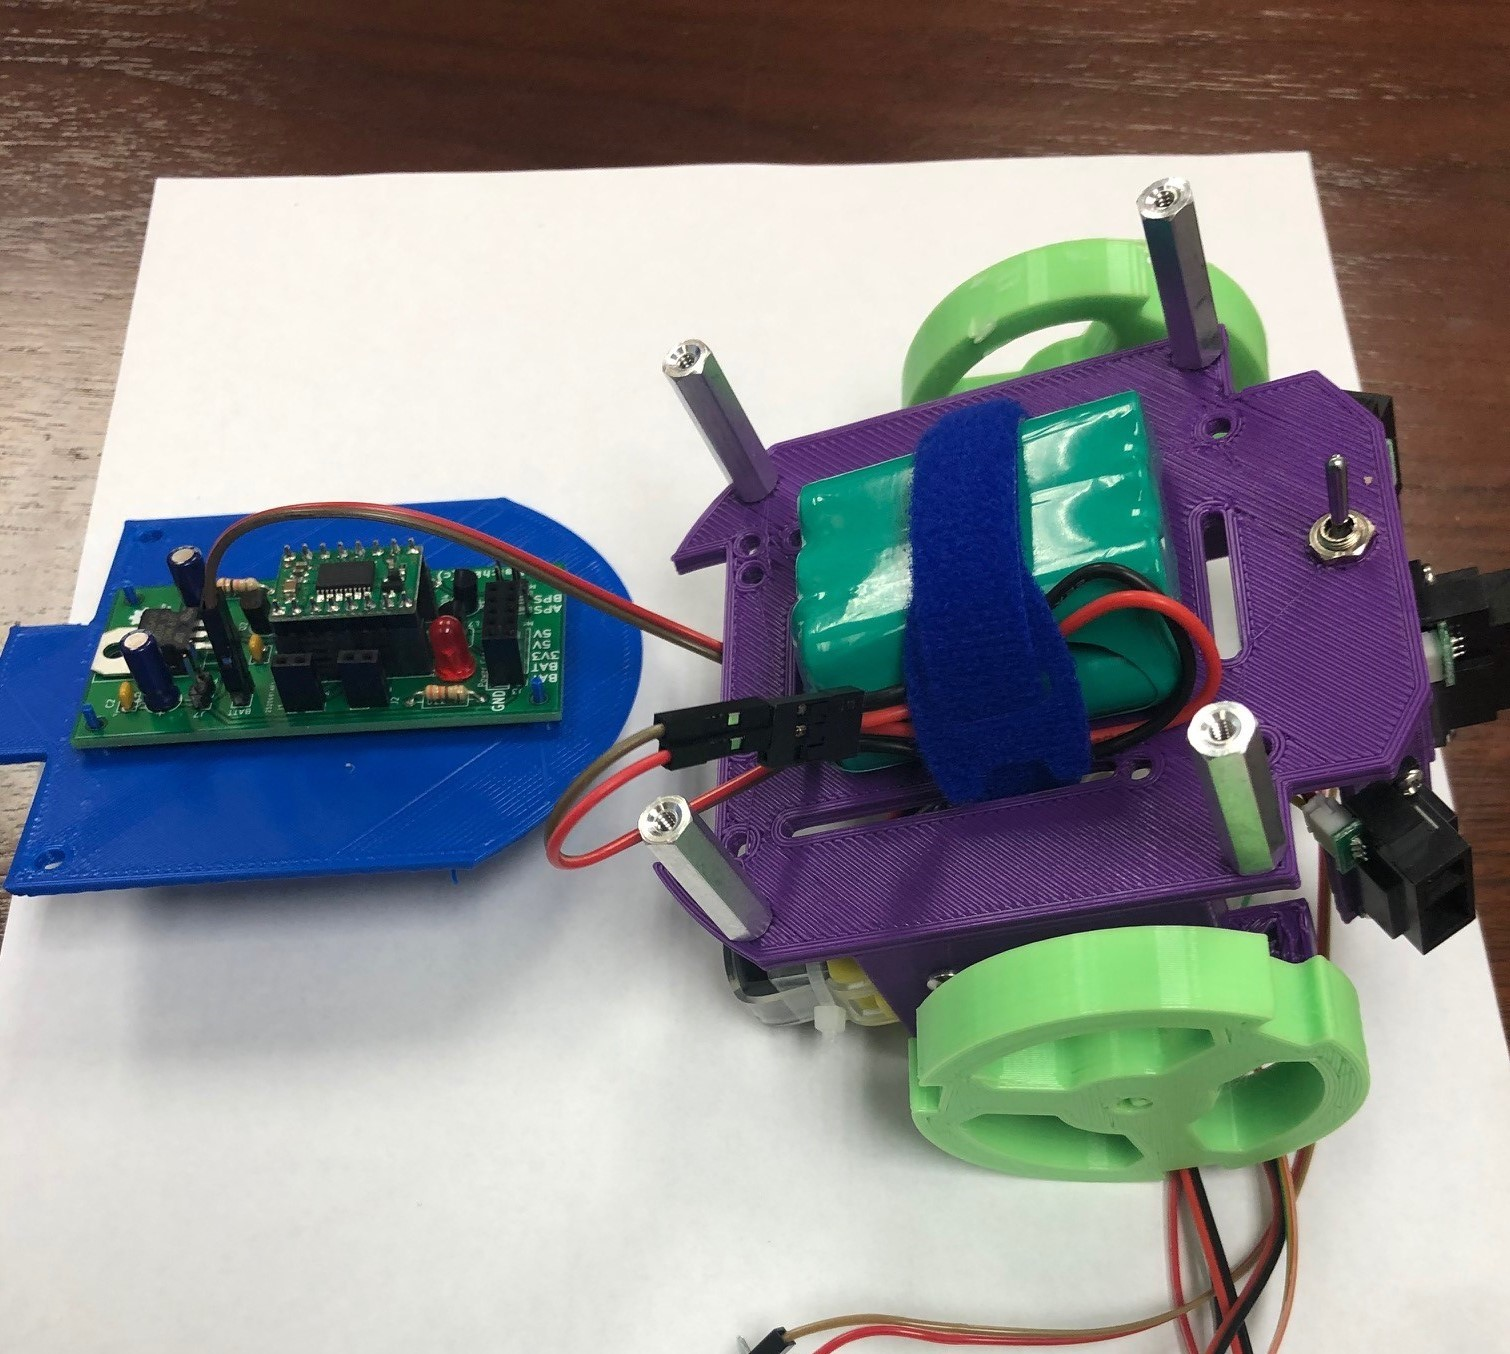
\includegraphics[width=.5\textwidth]{7.jpg}
		\end{figure}
		
	\end{enumerate}

	\section{Layer C - Arduino Layer.}
	\begin{enumerate}
		\item Connect Layer C to Layer B using the larger standoffs.
		\item Place the Arduino on the printed spacers (will only go one direction).
		\item Wire the Arduino to the PCB going through the slots in Layer C and B.
		\item Feed the wires from the IR sensors through the slots at the front of Layer B and C.
		
		\begin{figure} [H]
			\centering
			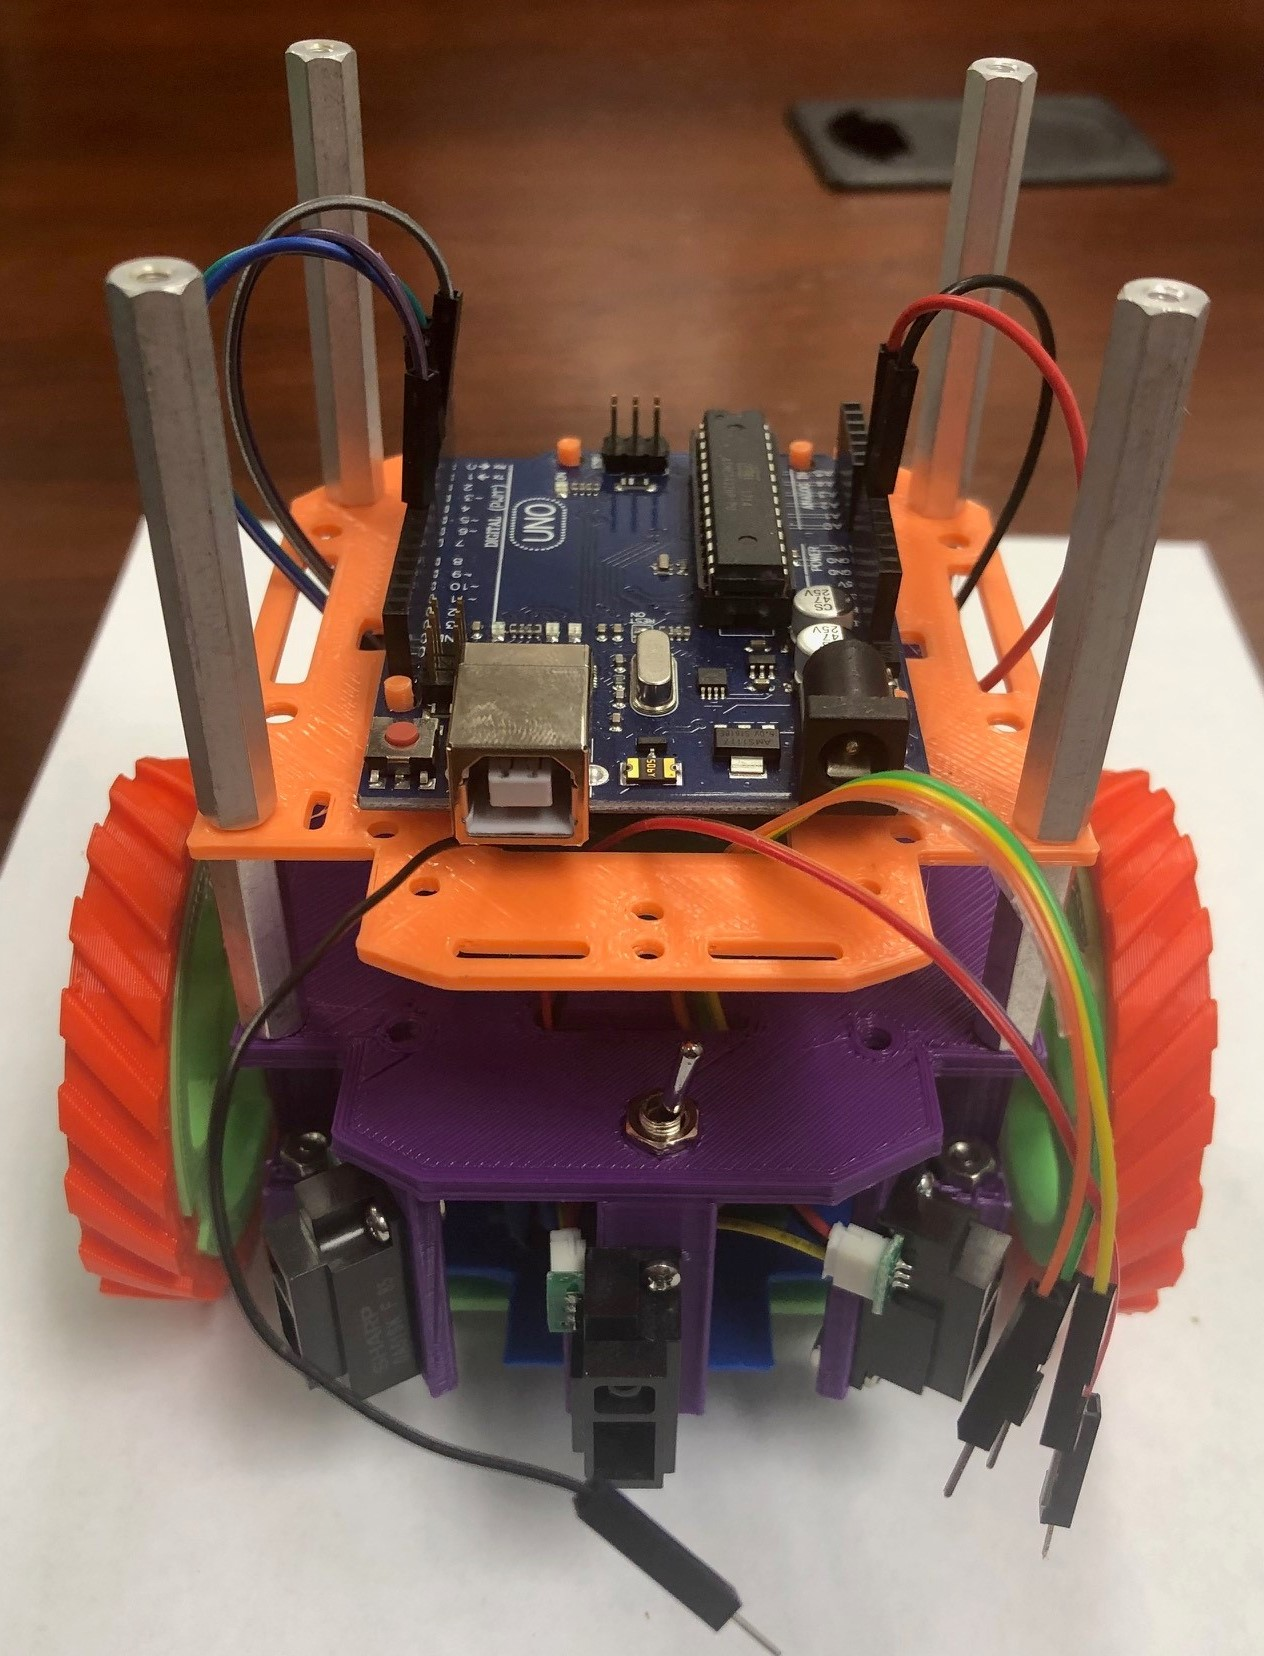
\includegraphics[width=.45\textwidth]{8.jpg}
		\end{figure}

	\end{enumerate}

	\section{Connect Layer A to Layer B/C.}
	\begin{enumerate}
		\item Connect the three layers using the line sensor mount and 2 - \# 4-40 x 1" bolts and nuts.
		
		\begin{figure} [H]
			\centering
			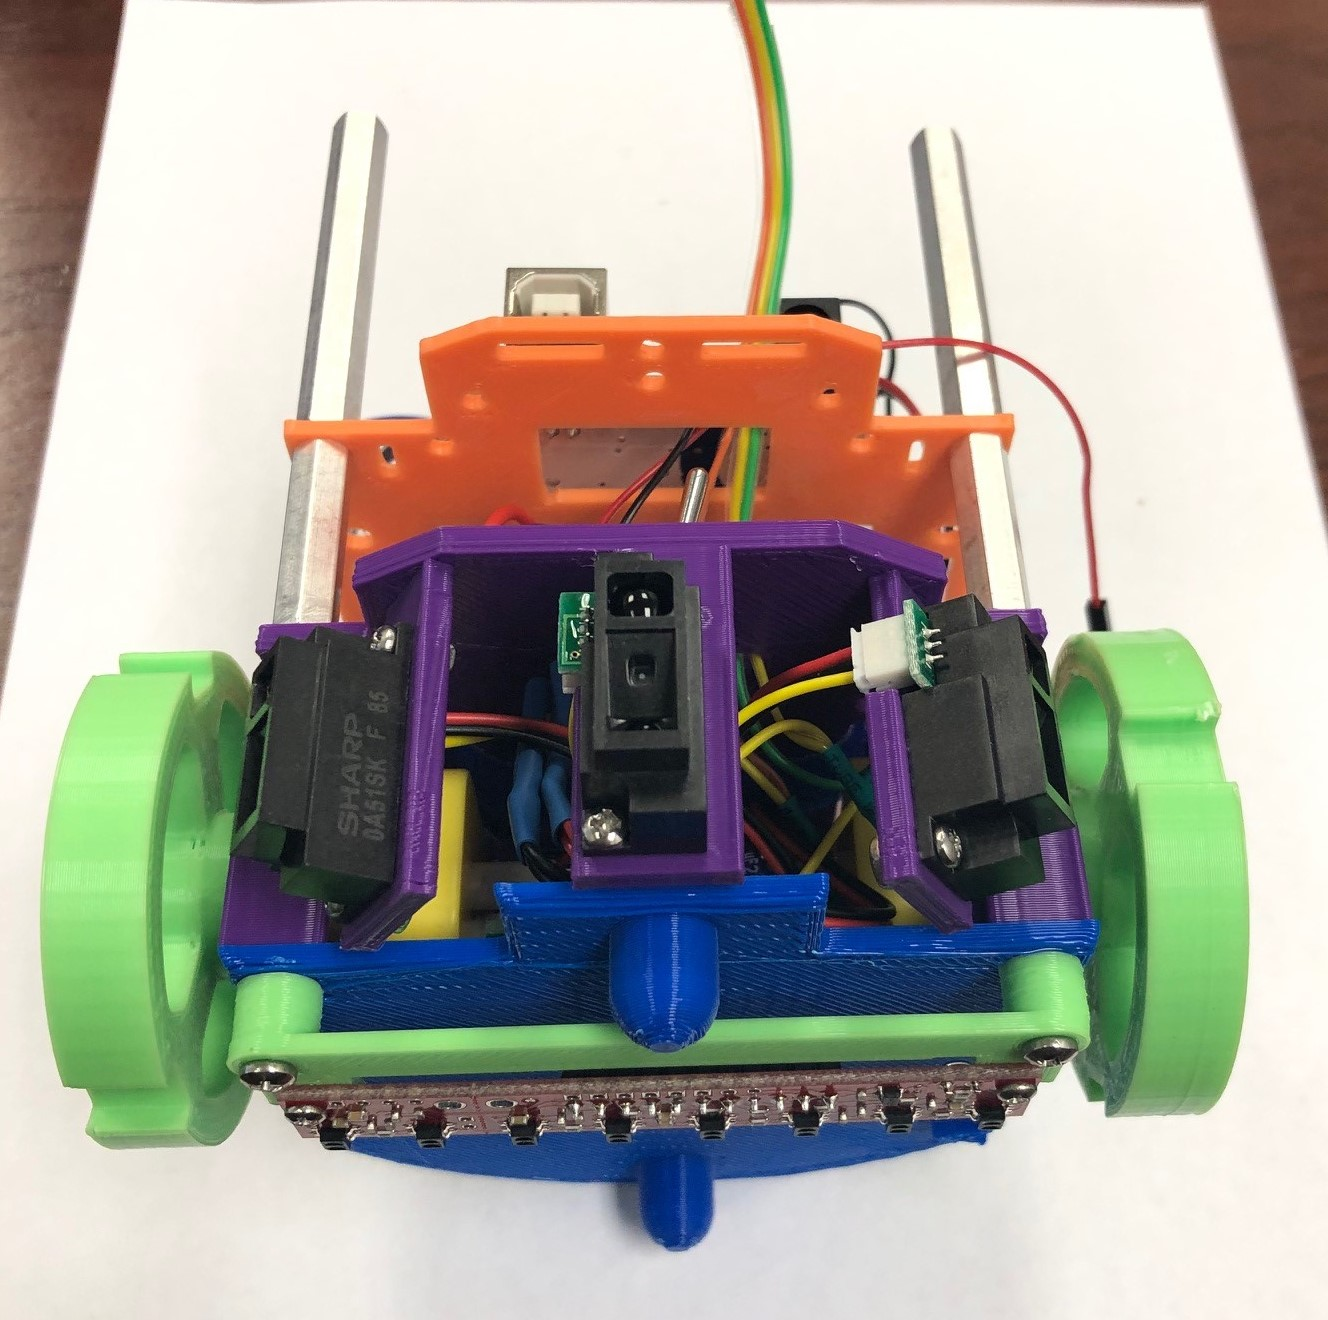
\includegraphics[width=.45\textwidth]{9.jpg}
		\end{figure}
		
		\item Put the tires on the wheels.
		
		\begin{figure} [H]
			\centering
			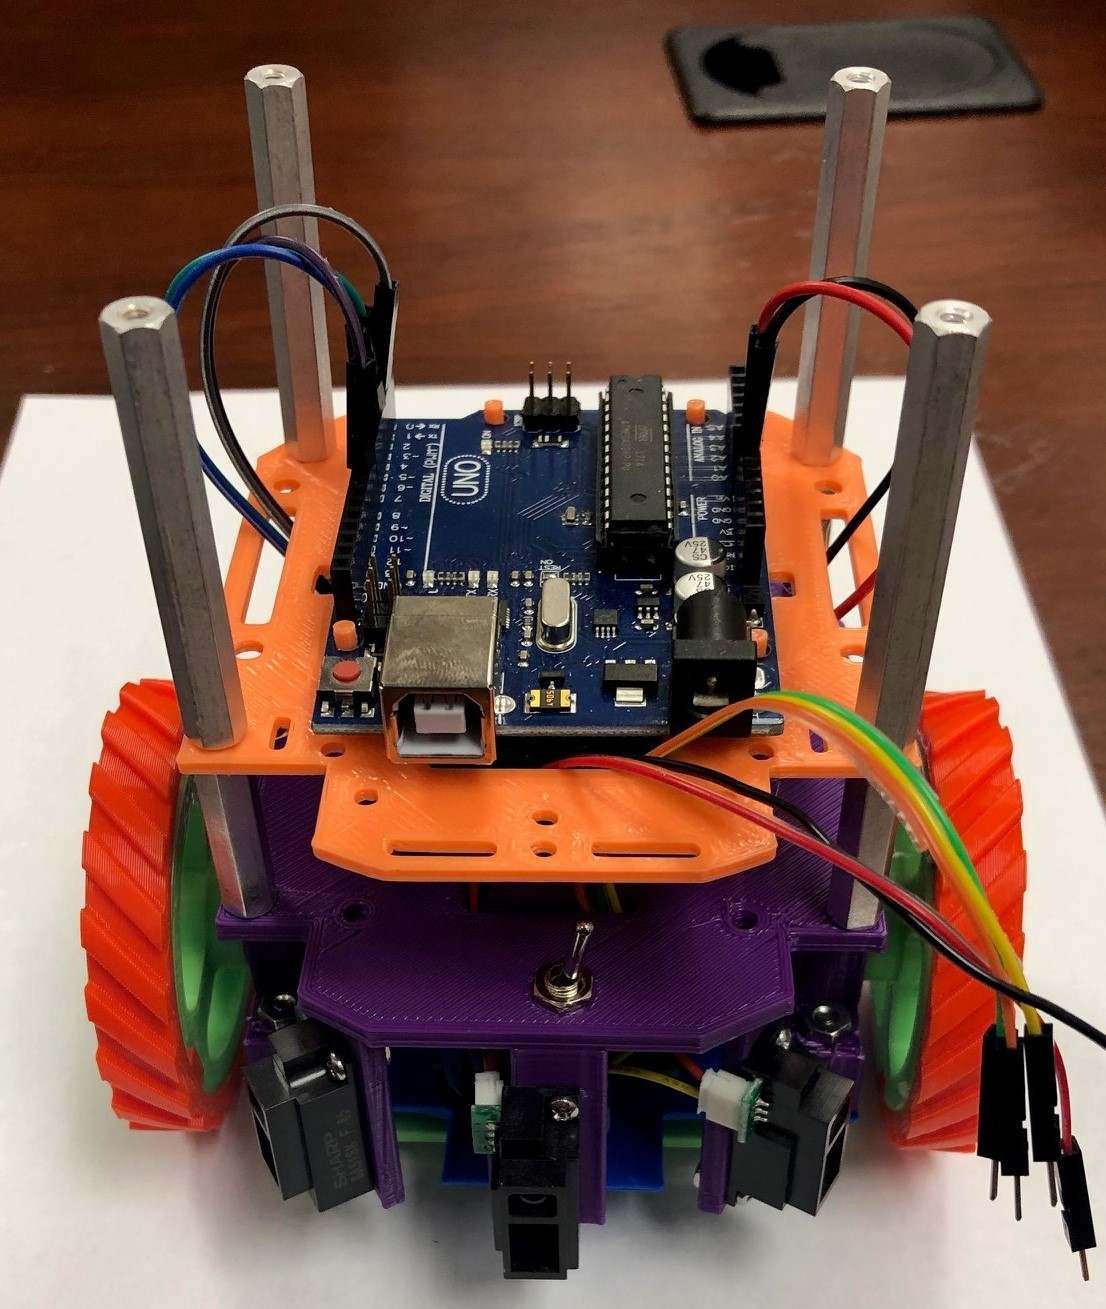
\includegraphics[width=.45\textwidth]{10.jpg}
		\end{figure}
		
	\end{enumerate}

	\section{Testing.}
	\begin{enumerate}
		\item Connect the battery to the jumper and turn on the PCB. The robot should drive in the same pattern as before.
	\end{enumerate}
		
		
	
	\newpage
	\clearpage
	\pagebreak
	
\end{document}
